\documentclass[a4paper]{article}
\usepackage{graphicx}

\begin{document}
% To add an image to the LaTeX file, you need to use figure environment and the graphicx package. Use \usepackage{graphicx} and
\begin{figure}
  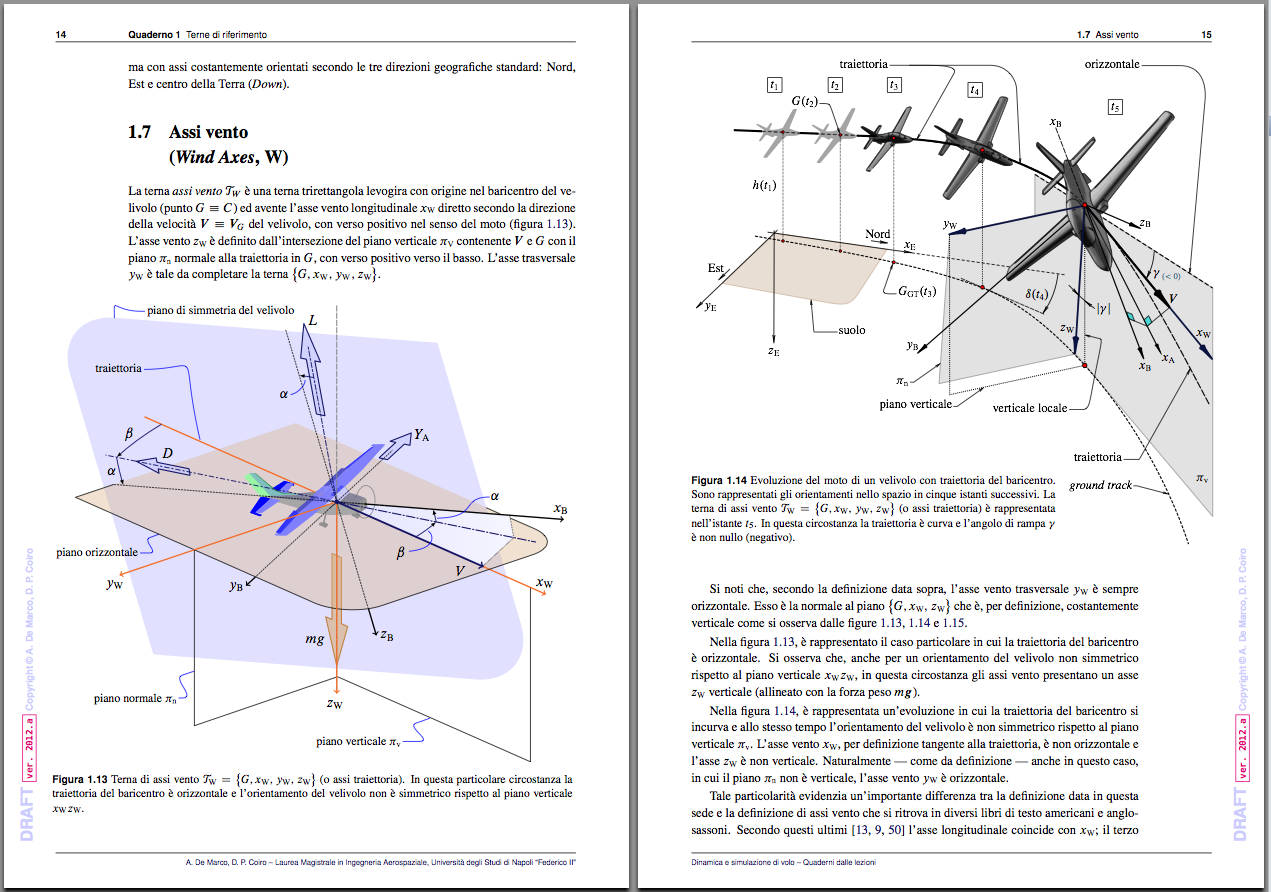
\includegraphics[width=\linewidth]{images/8IOMm.png} % Put [width=\linewidth] to scale the image to the width of the document.
  \caption{What is it about?}
  \label{fig:airplane}
\end{figure}
\begin{enumerate}
 \item How to have headers in margins (up to margin)
 \item Is it possible to start section headings from margin
 \item How to set figures occupy the margin
\end{enumerate}

\begin{figure}
  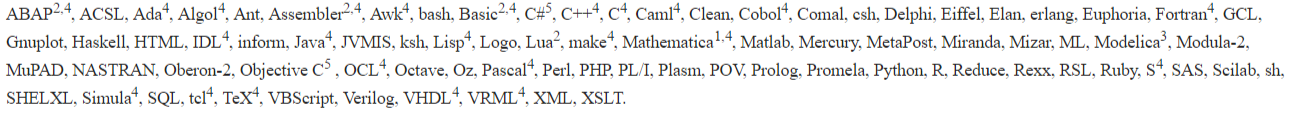
\includegraphics[width=\linewidth]{images/latex-language.png}
  \caption{LaTeX supports syntax for these languages}
  \label{fig:latex}
\end{figure}

\begin{figure}[p!]
  
\includegraphics[width=\linewidth]{images/latex.png}
  \caption{Latex}
  \label{fig:float-on an extra page}
\end{figure}
\end{document}
